\documentclass{article}
\usepackage{import}
\subimport{../}{preamble}
\begin{document}

\section{Optical Design}
\label{sec:optical_design}

\begin{figure}[p]
\centering
\fontsize{9.5pt}{1em}\selectfont
\def\svgwidth{0.93\textwidth}
\subimport{./figures/}{layout.pdf_tex}
\caption[Diagram of the full optical layout]{\textbf{Diagram of the full optical layout and specification of the microscope.} All optics are accounted for except for silver periscope mirrors, which transfer the beam between platforms of differing height and maintain the stronger $p$ polarisation oriented along the tip axis.}
\label{fig:layout}
\end{figure}

\Gls{df} spectroscopy is the primary optical method used to study plasmonic nanostructures, in which samples are illuminated at high angles with reflections filtered to collect only low-angle scattering from the focal plane. This microscope employs two kinds of DF microscopy - conventional DF imaging using a side-illumination fibre and supercontinuum (white light) laser DF spectroscopy.

The optical design employs the concept of reimaging spatial filters into the correct planes for efficient DF spectroscopy, leading to a compact design. Employing reimaging means that beams are not necessarily required to propagate exactly along the optical axis, minimising the number of long, empty beam lines, typically used for alignment. By reimaging the front and back focal planes of the objective, spatial and Fourier filters are placed in the corresponding planes, ensuring optimum filtering performance and minimal aberration. A detailed schematic of the microscope platform and the surrounding optical bench layout, containing the specifications of all optics used, is found in \figurename~\ref{fig:layout}.

% Reimaging for compactness
Both image and Fourier planes are set through careful placement of each set of lenses. The required minimum degrees of freedom for beam alignment are accounted for by mirrors placed in the focal and Fourier planes. Those in Fourier planes change the position of the beam without affecting it's shape, whereas those placed in focal planes only change the beam shape without shifting the position in the objective focus.%
\footnote{Diagrams indicating the principles of beam alignment using reimaging are found in the appendices.}
The position and shape of the beam are therefore independently adjustable, greatly simplifying beam alignment. This advantageous technique results in a high beam quality, and, as a direct result of the lack of long, iris-containing beam lines, a compact microscope.

% The objective and illumination collar
A long working distance objective is required for imaging and spectroscopy of tips. Additionally, a large \gls{na} is required to properly study nanostructures as it means light is collected across a large acceptance angle with a small focal length and large magnification. A \gls{bf} long working distance IR objective (Olympus LMPlan 100$\times$ IR, 0.8\,NA) is used to access wavelengths above \SI{700}{nm}, for which the more convenient DF VIS objectives (Olympus LMPlan 100$\times$ BD) exhibit a sharp cutoff.%
\footnote{A comparison of the two available 100$\times$ objectives is found in the appendices.}
A DF illumination/collection configuration is necessary for imaging scattered light from a nanostructure. Since DF illumination is not supported on BF IR objectives, light needs to be brought in externally in a side-illumination geometry to image samples. A 3d-printed objective collar is used to hold a \SI{1}{mm} diameter optical fibre approximately \SI{1}{mm} from the sample, outside of the objective collection angle, to which a cold white LED is fibre coupled. The fibre is fed through a breadboard hole in the top plate and sealed so as to preserve the environmental chamber integrity. The fibre outputs a broad cone of light which illuminates samples over a large area.

% Fianium source and power control
Use of a ultra-high brightness supercontinuum laser source (Fianium SC-400, \SI{4}{W}, 480--\SI{1750}{nm}) enables single nanostructure spectroscopy with exposure times around 10--\SI{50}{ms}. The beam is expanded to fill the back aperture of the objective and apertured into a ring to mimic DF illumination using a DF disc stop placed in a Fourier plane. The inner diameter of the ring is set at \SI{2}{mm} and the outer diameter is set by the back aperture of the objective, in this case \SI{3}{mm}. This technique is a pseudo-DF method denoted \gls{sdf}. % Does this need justifying
To prevent laser damage to samples the incident power is heavily attenuated. Reflective neutral density filters totalling ND\,1.6 (2.5\% transmission) are placed in the beam line to reduce the initial incident power. The majority of the incident power is lost at the DF stop. Further attenuation results from the 10:90 (R:T) beamsplitter used to relay the laser into the microscope. At this point the total power integrated over the whole spectral range is reduced to around \SI{1}{mW}, as measured on a bolometer (Coherent, Inc.) behind the objective. Whilst the power is seemingly low and comparable with high-brightness incoherent light sources, the focussing ability of the single mode laser results in an intense, diffraction-limited, white light focus not possible with incoherent sources. For an assumed broadband spot size around \SI{1}{\micro\metre} the focal intensity is $\sim${\SI{e5}{\watt\per\centi\metre\squared}}.

% Reimaging technique
The incident light is apertured and reimaged directly onto the back focal (Fourier) plane of the objective, as opposed to aperturing close to the objective back aperture. This prevents diffractive artefacts in the conjugate plane of the collected light. The ring aperture means that the focus is illuminated only at high-NA as with conventional DF spectroscopy. Scattered light is then filtered by a DF iris placed in a Fourier plane in the returning beam path to remove any signal contribution from reflected, high-NA illumination. Reimaging allows both the DF iris and stop to be located away from the objective for convenient access and easy adjustment. Alternative designs using optics mounted at the objective back aperture do not benefit from having the stop and iris in conjugate planes and may require motorised irises if not accessible by hand. For this experiment a simple graduated dark-field iris is sufficient for external use to filter the collected light signal.

% Collection efficiency
Since incident power is not an issue, and in many cases requires significant attenuation, the microscope is optimised for efficient collection. The 10:90 beamsplitter used for laser input means only 10\% of collected light is lost when returning back through the main microscope arm. Furthermore, all optics in the system are optimised for light between 500--\SI{1100}{nm}.%
\footnote{Broadband optimisation is achieved via exclusive use of Ag mirrors, Edmund Optics VIS-NIR AR coating on lenses, COMAR NIR and ThorLabs visible or visible-NIR coated beamsplitters.}
The angle-dependent Fresnel coefficients of the glass used in all optics components mean that $p$-polarised light is favoured during transmission throughout the microscope collection path.%
\footnote{All beamsplitters have some degree of polarisation sensitivity due to Fresnel coefficients of the glass used. Reflectance can be a factor of 2 different between orthogonal linear polarisations. A comparison of polarisation-dependent reflectances is found in the appendices.}
A \SI{90}{\degree} turning periscope is placed after the first reimaging lens to reverse the linear polarisations of light so that the stronger $p$-polarisation component is orientated along the tip axis.

% CCD imaging and spectroscopy
Subsequently, collected light is split into imaging and spectroscopy paths using a second (50:50) beamsplitter placed before the DF iris. CCD imaging is both used to align and characterise the laser focus and to centre samples onto the targeted laser illumination spot. Sample imaging uses light collected from the scattered white LED side-illumination light to produce DF images whereas laser light is not DF-filtered in this path. Images are magnified 111$\times$.%
\footnote{Magnification is calculated by the ratio of focal lengths, $M=f_2/f_1$.}
Light passing along the spectroscopy path is DF-filtered to remove any contributions to the scattering signal from reflected light. A graduated iris is used to remove the \SI{2}{mm} outer ring of the returning beam. The iris is placed in the image plane of the DF stop for the most accurate filtering and optimum performance. The two beamsplitters present before the DF iris are wedged to prevent ghost images, which transmit through the closed iris and create spectral artefacts. However, the \SI{5}{mm} thickness of wedged beamsplitters means increased dispersion and the limited availability of broadband AR coatings results in reduced reflectance in the NIR. %This, however, only affects CCD imaging, which is limited to visible wavelengths only.
Additionally, the DF-filtering process only works to remove light reflected out at the same angle. Angled samples (such as the facets of tips) can reflect light into the low-NA collection, creating spectral artefacts. It is for this reason that the flat tip facets are even visible in a dark-field configuration.

\subsection{Confocal Localisation of Spectra}

% Confocal filtering
\begin{figure}[bt]
\centering
\fontsize{10pt}{1em}\selectfont
\subimport{./figures/}{confocal_diagram.pdf_tex}
\caption[Diagram of optical sectioning in confocal microscopy]{\textbf{Diagram of optical sectioning in confocal microscopy.} (a) Out of focus light from nearby focal planes leads to blurring and a decrease of contrast in images. (b) Images spatially filtered in the focal plane by a confocal pinhole localise light from only a select volume that is sufficiently focussed to pass through the pinhole aperture, improving both contrast and resolution.}
\label{fig:confocal_diagram}
\end{figure}

Since the laser focusses to a diffraction-limited spot on the sample, spectra are collected from a small sampling volume. This single mode input forms the first component of confocal localisation. Further spectral localisation is achieved by confocally filtering the image plane after the DF iris using a \SI{25}{\micro\metre} pinhole to collect light from only the central focal spot. Only light in focus on the pinhole may pass through it. By rejecting out of focus light the image becomes an optical section with a tighter depth of focus. The size of the pinhole sets both the lateral and axial width of the transmitted light and leads to both spatial masking and optical sectioning in the objective-sample plane, as shown in \figurename~\ref{fig:confocal_diagram}. Spectra are therefore acquired from a localised sampling volume, as set by the location of the 47$\times$ demagnified pinhole image. The location of this spatial mask image in the objective focus is controlled by a mirror before the confocal filtering array. A slip-in small CCD is used to image the Fourier plane before and after confocal filtering to check pinhole alignment. Since the depth of focus scales as $M^2$ (or $\NA^2$) the placement of the pinhole along the beam path is not critical. Choice of pinhole diameter, however, is important.

Confocal filtering not only improves image contrast but also improves upon the wide-field, diffraction-limited resolution by up to a factor of $\sqrt{2}$, depending on pinhole diameter, at the cost of image brightness \cite{webb1996confocal, murphy2002fundamentals, cox2004practical, hollricher2011high}. This stems from the removal of higher diffraction orders by the pinhole. The resolution of a microscope is often quantified using the Rayleigh criterion - the distance from the maximum of the \gls{psf} (expected to be an Airy function) to the first minimum  \cite{born1999principles}. A decrease in the Rayleigh criterion of diffraction-limited resolution is expected, going from $\gls{r_lat}=0.61\lambda/\NA$ down to $r_{\mathrm{lateral}}=0.44\lambda/\NA$ at best.
Decreasing the pinhole diameter therefore not only decreases the optical section thickness but also the minimum resolvable lateral distance to a certain extent.

\begin{figure}[bt]
\centering
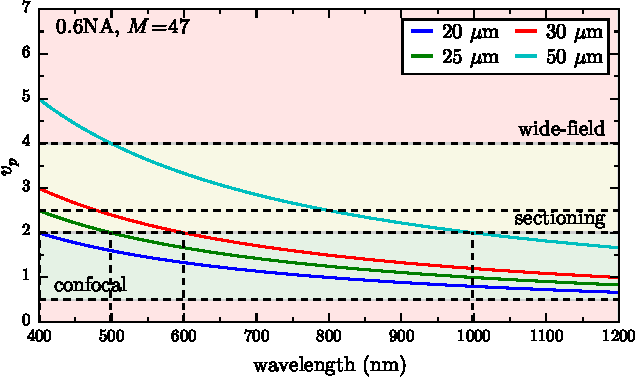
\includegraphics{figures/confocal_pinhole_choice}
\caption[Calculated optimum confocal pinhole size across the visible-NIR spectrum]{\textbf{Calculated optimum confocal pinhole size across the visible-NIR spectrum.} The detector width $v_p$ determines the performance of confocal imaging, for which the characteristic detection regimes are highlighted. A \SI{25}{\micro\metre} pinhole is chosen for most experiments. Confocal performance is then achieved above \SI{500}{nm} with significant intensity losses above \SI{1000}{nm}.}
\label{fig:confocal_pinhole_choice}
\end{figure}

For a realistic detector aperture the collection PSF is convoluted with its aperture function, $D_p$, giving an image \gls{psf} $I=|h_1|^2(|h_2|^2 \ast D_p)$, where $h_1$ is the excitation PSF and $h_2$ is the detection PSF \cite{wilson1987size}. The resulting resolution depends on a quantity $v_p$, the detector width, which can be related to the actual pinhole diameter, \gls{pinhole}, through \cite{wilson1987size},
\begin{equation}
	v_p \geq \frac{\pi d_p \NA}{M \lambda}.
\end{equation}
The \gls{fwhm} of the PSF retains the full, $\sqrt{2}$ improvement if $v_p\leq0.5$, but this leads to a significant loss in brightness. An increased resolution is still in effect until $v_p\geq4$, at which point the wide-field behaviour is recovered. Practically, $v_p\leq2$ for optimal lateral resolution and image brightness, and $v_p\leq4$ for optimal depth resolution. Optimising for $v_p=2$ means that for a 0.6\,NA, $M=47$ system (the spectroscopy collection geometry) $d_p/\lambda\leq43$, i.e.\ \SI{25}{\micro\metre} at \SI{500}{nm} and \SI{55}{\micro\metre} at \SI{1100}{nm}. A plot of $v_p$ across the visible-NIR spectrum for a number of pinholes is shown in \figurename~\ref{fig:confocal_pinhole_choice}, highlighting the relevant confocal regimes. For a given pinhole size that acts confocally in the visible, the intensity of some NIR wavelengths will be reduced since $v_p$ drops below 1, however this loss is acceptable to maintain higher resolution in the visible region of the spectrum. A \SI{25}{\micro\metre} pinhole size is determined to be optimal in this microscope based on this analysis and the range of available pinhole sizes.

% Spectroscopy in general
Once filtered only the spectral content of the beam is of interest rather than the image so strict adherence to conjugate planes is no longer necessary. The beam is split 50:50 into two signals, with one going to the benchtop spectrometers and the other to a fast spectroscopy path.%
\footnote{The fast spectroscopy technique is developed and implemented but otherwise not used in any experiments in the current project. For this reason it's operation is omitted from the main text. A brief discussion of its implementation can be found in the appendices.}
% Spectroscopy arm
The benchtop spectroscopy signal is further split into linear $s$ and $p$ polarisation components using a broadband polarising beamsplitter cube (Melles-Griot 300--\SI{1100}{nm}). Broadband polarisers (Thorlabs 500--\SI{1500}{nm}) oriented along the $s$ and $p$ axes are placed at the cube output ports to increase extinction. Each polarised signal component is then finally focussed into multi-mode fibres, using short focal length (\SI{11}{mm}) lenses to achieve a spot size smaller than the fibre core. \SI{100}{\micro\metre} fibre core is used instead of \SI{50}{\micro\metre} to reduce laser speckle in spectra since the confocal pinhole diameter already localises the signal.
% Spectrometers
The spectral signal from each of the fibres is recorded using TE-cooled, benchtop spectrometers (Ocean Optics QE65000 and QE Pro) with integration times between 10--\SI{50}{ms}. The sensitivity of the Si detectors in the spectrometers drops off beyond \SI{900}{nm}, imposing a limit to detectable signals of around \SI{1100}{nm}. The supercontinuum laser imposes a \SI{480}{nm} spectral short wavelength cut-off, resulting in an overall effective measurement window of 500--\SI{1100}{nm}.

%\subsection{Measuring Spectra}
Measured spectra are background-subtracted, to remove dark counts, and referenced to the spectral density of the supercontinuum illumination as transmitted through the microscope optics. Use of the intense supercontinuum source means low integration times below \SI{20}{ms} are sufficient to near saturate the spectrometer for a high quality signal to noise. The high brightness of the supercontinuum laser at these exposures also means that the relative intensity contribution from external light sources is negligible.
The coherence of the supercontinuum laser means that conventional referencing using scatter from a white diffuser to map the illumination spectral density is not possible. Instead, reflections from thin, reflective substrates attached underneath the piezo-mounted tip mount are used as a reference. Different substrates are used depending on the sample. For metallic samples the substrate is matched to the metal so only structural spectral features are observed. Otherwise either a Ag mirror or glass slide are sufficient for referencing as they provide relatively flat reflectances across the visible-NIR spectrum. The DF iris is kept fully open during reference acquisition to ensure the full spectral content of the incident beam is measured and to avoid introducing referencing artefacts. As optics are very rarely broadband between 500--\SI{1100}{nm}, all non-essential pathways are closed when acquiring spectra to prevent artefacts. Back reflections off lenses are found to superimpose a weak duplicate of the illumination spectrum onto spectra since the reflections are translated in the Fourier plane and are therefore not completely filtered by the DF iris.

\subsection{Characterisation of Microscope Performance}

% Power measurement and beam profiling
During most experiments the power incident on samples is kept below \SI{1}{mW} corresponding to a focal intensity of $\sim$\SI{e5}{\watt\per\centi\metre\squared}. This is used to maintain sufficient signal quality whilst preventing damage or destructive changes to nanoscale Au samples (typically \SI{50}{nm} Au coatings). Beam profiling, the study of the beam shape through the focal volume, is used to characterise beam propagation in the microscope and determine its ability to collect DF spectra. Profiling is carried out using focal scans of both light reflected from a Ag mirror and light scattered from an \SI{80}{nm} AuNP, measured simultaneously on a CCD and a spectrometer. The CCD is used to laterally profile the beam through the focus while the spectrometer characterises the confocal profile and spectral distribution of the light. Both the illumination and collection pathways are profiled. The illumination pathway is profiled using the DF-filtered supercontinuum beam while one of the collection fibres is removed from its spectrometer and coupled to a \SI{532}{nm} single mode laser in order to profile the collection pathway.

\begin{figure}[bt]
\centering
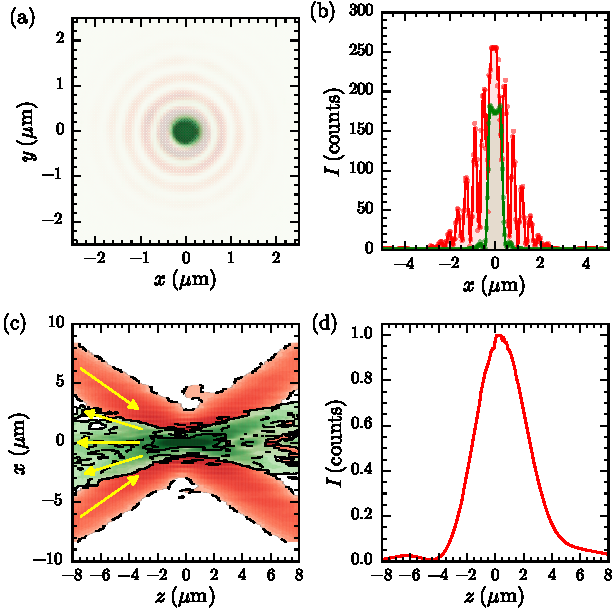
\includegraphics{figures/beam_profile}
\caption[Beam profiling of supercontinuum illumination and scattering collection beam lines.]{\textbf{Beam profiling of dark-field filtered supercontinuum illumination (red) and scattering collection (green) beam lines.} Supercontinuum laser light is reflected back from a Ag mirror in the objective focus to characterise the illumination pathway. The spectroscopy pathway is characterised by coupling a \SI{532}{nm} laser into a single mode fibre and passing it through the collection optics with the DF-iris closed to \SI{2}{mm}. The stated axial distance $z$ is twice the displacement of the mirror to account for reflections to the focal plane. Lateral distances are calculated using the CCD array size and pixel dimensions. (a) Lateral beam profile of the illumination and collection focusses as measured on the CCD. (b) Intensity cross sections through the lateral beam profiles of the illumination and collection. (c) Axial cross section through the focus of illumination and collection beams. (d) Normalised summation of spectrometer counts of confocally localised supercontinuum light passing through the collection optics.}
\label{fig:beam_profile}
\end{figure}

% Discussion of beam profiling in terms of dark-field spectroscopy technique
\figurename~\ref{fig:beam_profile} shows both the lateral focal spot on the CCD and relevant cross sections along the optical and focal axes for both the illumination and collection optics, along with depth-profiling using broadband-integrated spectra. \figurename~\ref{fig:beam_profile}a shows the beam structure in the focus.  The single mode fibre output exhibits the characteristic Airy profile expected of a reimaged beam while the ring aperture of the supercontinuum beam leads to more power concentrated in the outer rings of the focal pattern (\figurename~\ref{fig:beam_profile}b). The measured FWHM of the collection beam is \SI{460\pm20}{nm} with a beam waist ($1/\e$ width) of \SI{540\pm20}{nm}. The 47$\times$ demagnified image of the \SI{25}{\micro\metre} pinhole is expected to be \SI{530}{nm}. The focal radius of a single mode Gaussian beam  (the beam waist) is given by $w_0 = \lambda/\pi\NA$, which results in a collection NA of \num{0.62\pm0.02}. Measurement of a Rayleigh criterion length of \SI{530\pm20}{nm} indicates the beam is focussed through \num{0.61\pm0.02}\,NA. Uncertainties on these calculations of the NA are small since the \SI{532}{nm} wavelength is well known. Both calculations of the NA only partially agree due to beam focussing at the diffraction limit and both show a collection half-angle of \SI{38.0\pm0.5}{\degree}.

%The \gls{psf} defines the overall diffraction-limited focal pattern of the microscope. Multiplying the illumination and collections focal patterns and measuring the width defines the resolution of the system. The measured FWHM of the central illumination beam is \SI{360\pm20}{nm} with a beam waist of \SI{430\pm20}{nm}. The NA of the microscope calculated from the beam waist is \num{0.80\pm0.02}, exactly as quoted on the objective.

The axial cross section of beams (\figurename~\ref{fig:beam_profile}c) shows the focussing of the high angle (0.64--0.8\,NA, 40--\SI{53}{\degree} incident angle) supercontinuum ring. The boundary between incident and collection beams is measured to be around 0.62 in both beam angle and spot size measurements since the DF iris diameter and the DF stop diameter are both set to \SI{2}{mm}. The axial beam profile, however, measures the angle of light from the focus to below \SI{21\pm1}{\degree} (0.35\,NA). This is likely caused by observation error due to the low intensities at high angles. After confocally filtering the depth of focus, as measured on the CCD beam profile, is on average \SI{4}{\micro\metre} across the supercontinuum wavelength range (\figurename~\ref{fig:beam_profile}d).

% Axial chromatic aberration
\begin{figure}[bt]
\centering
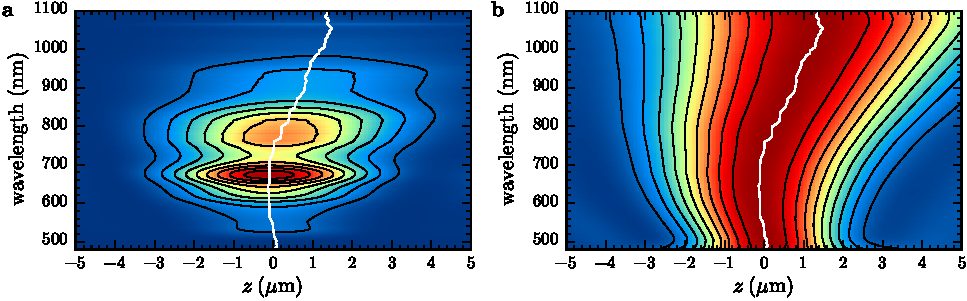
\includegraphics{figures/axial_chromatic_aberration} % maybe wants contour lines on to improve
\caption[Axial chromatic aberration at each wavelength through the objective focus]{\textbf{Axial chromatic aberration at each wavelength through the objective focus.} The image in (a) is formed from spectra of the $s$-polarised component of a reflection from a Ag mirror scanned through the focus. An intensity plot normalised at each wavelength is shown in (b) to determine depth of focus. The white indicates the position of maximum signal along the optical axis for each wavelength and shows the distinctive bowing curve of chromatic aberration.}
\label{fig:axial_chromatic_aberration}
\vspace{-5pt}
\end{figure}

\figurename~\ref{fig:axial_chromatic_aberration} shows the individual wavelength components that make up the integrated spectral signal in \figurename~\ref{fig:beam_profile}d. As expected the depth of focus increases with wavelength. The depth varies from \SI{2.8\pm0.1}{\micro\metre} at $\lambda=\SI{500}{nm}$ to \SI{6.4\pm0.1}{\micro\metre} at $\lambda=\SI{1100}{nm}$. The chromatic structure of the beam is non-linear and shows that the colour maxima for $\lambda<\SI{550}{nm}$ and $\lambda>\SI{800}{nm}$ occur slightly offset from the pinhole position. Overall this does not detract much from the measured spectra since intensity differences in the chosen focal plane are normalised with the reference spectrum.

% AuNP hyperspectral scans show lateral localisation vs. pinhole diameter
\begin{figure}[bt]
\centering
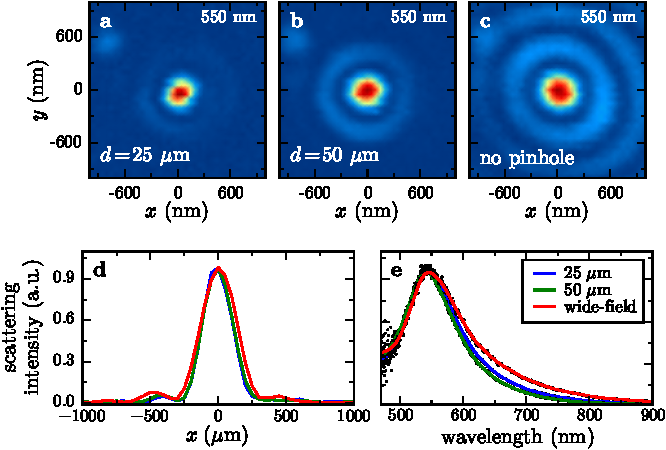
\includegraphics{figures/lateral_aunp_scans}
\caption[Hyperspectral scans of a AuNP used to characterise the lateral PSF with different confocal pinhole diameters.]{\textbf{Hyperspectral scans of a AuNP used to characterise the lateral PSF with different confocal pinhole diameters.} (a-c) Wavelength slices of AuNP scans on resonance using \SIlist{25;50}{\micro\metre} diameter pinholes and finally no pinhole, respectively. (d) The extracted PSF from line profiles across  images (a-c). (e) Spectra of imaged AuNPs at the scattering centroid location. Localisation is observed with reduced pinhole diameter as the concentric illumination rings are cut.}
\label{fig:lateral_psf}
\end{figure}

Lateral localisation is more important to consider than axial sectioning. Scattered light from a sub-wavelength size nanoparticle provides a point source from which the PSF can be measured across a small, resonant bandwidth. By (raster-) scanning a strongly-scattering MNP under the beam its point scattering response is convoluted with the beam structure in the focus. The size of the confocal pinhole determines how much of this beam structure is laterally filtered prior to spectroscopy and thus, by measuring the scattering spectra, the actual PSF, as seen by the spectrometers, can be mapped across a broad range of wavelengths. It is this function that determines the specific locations from which spectra are collected and becomes particularly important when attempting to measure localised scattering from an extended nanostructure.

\figurename~\ref{fig:lateral_psf} shows scattering profiles extracted from AuNP scans, demonstrating the effective spectral PSF for a range of pinhole diameters. \SI{80}{nm} AuNPs on glass resonantly scatter at \SI{550}{nm} due to excitation of the dipolar LSP. A single AuNP was chosen on which multiple scans were performed, changing and realigning the confocal pinhole in between each scan. Wavelength slices at the AuNP plasmon resonance (\figurename~\ref{fig:lateral_psf}a--c) show the effective lateral PSF. Without a pinhole in place the spectral PSF is a convolution of the focal beam profile shown in \figurename~\ref{fig:beam_profile}a. The spectrometer sees the scattering from each of the concentric rings in the focus so localisation of spectral features to the beam centre cannot be guaranteed. Decreasing the pinhole diameter filters scattering from the focus and removes the contributions to spectra from the outer rings until spectra can only be acquired from the central spot. This guarantees localisation of observed spectral features to a finite-sized region. The FWHM of the scattering signals on resonance are \SI{255\pm25}{nm} with the \SI{25}{\micro\metre} pinhole in place, \SI{260\pm25}{nm} with the \SI{50}{\micro\metre} pinhole in place, and \SI{300\pm25}{nm} without a pinhole.
%A theoretical minimum FWHM of \SI{215}{nm} could be expected based on the wide-field result, however \SI{250}{nm} with a \SI{25}{\micro\metre} pinhole is more than acceptable and ensures good signal throughput.
The FWHM at \SI{900}{nm} for the case of the \SI{25}{\micro\metre} pinhole is \SI{410\pm25}{nm} for reference. Due to the single AuNP being the only source of scattering in each of the scans the measured spectrum is the same for all pinholes (\figurename~\ref{fig:lateral_psf}e). Though the resolution is not improved by a great amount, use of the smaller pinhole does guarantee better spectral localisation, as seen by the presence of only the central maximum in its PSF.

% Lateral chromatic aberration as measured by monitoring the AuNP PSF vs. wavelength
\begin{figure}[bt]
\centering
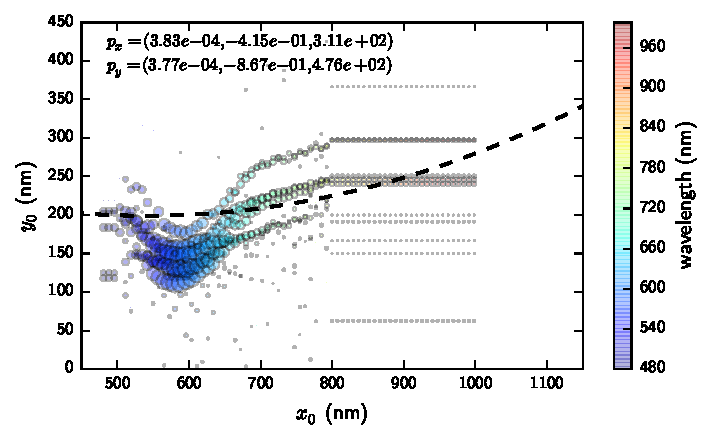
\includegraphics{figures/lateral_chromatic_aberration}
\caption[Measurements of lateral chromatic aberration across the plasmon resonance scattering bandwidth of a hyperspectrally imaged AuNP.]{\textbf{Measurements of lateral chromatic aberration across the plasmon resonance scattering bandwidth of a hyperspectrally imaged AuNP.} The centroid position of the optical scattering is extracted from images at each wavelength. Changes in centroid position with wavelength signify chromatic aberration. Displacements are scaled relative to the centroid position on resonance where the signal is highest.}
\label{fig:lateral_chromatic_aberration}
\end{figure}

Determining the centroid at every wavelength in the spectral data cube identifies lateral chromatic aberration in the microscope. This is an important parameter to consider when using hyperspectral imaging or when acquiring spectra. For example, if the chromatic aberration is systematic and fitted then a correction offset can be added to hyperspectral data cubes at each wavelength. Spectra from each pixel can then be further recombined into regular RGB images by integrating the spectra at each pixel with RGB pixel spectra.

\figurename~\ref{fig:lateral_chromatic_aberration} shows the centroids of the PSFs across the plasmon resonance band for each pinhole diameter. Scattering centroids are extracted from each wavelength slice using discrete image moment analysis,
\begin{equation}
	M_{ij} = \sum_x \sum_y x^i y^j I(x,y),
	\label{eq:image_moments}
\end{equation}
where $i,j$ denote the moments of the $x,y$ axes.%
\footnote{Note that the discrete image moments are based on the continuous moment theorem with moments given by $$M_{ij} = \int_{-\infty}^{\infty} \int_{-\infty}^{\infty} x^i y^j f(x,y) dx dy.$$}
The position of maximum scattering is then given by,
\begin{equation}
	(\bar{x},\bar{y}) = \left( \frac{M_{10}}{M_{00}}, \frac{M_{01}}{M_{00}} \right).
	\label{eq:centroid_position}
\end{equation}
The centroid position drifts almost linearly by \SI{80}{nm} in both the $x$ and $y$-directions. Since the pinhole only filters the outer rings of the PSF there is very little difference in the centroid positions between pinholes. As the range of centroid displacement in each direction is well below the diffraction limit and corresponds to only a few pixels offset in each image, the aberrations are not considered to negatively impact spectroscopy. % Should the magnification be taken into account

% Summary
To summarise, a microscope platform has been designed to accommodate various sample geometries, though with a specific focus on AFM tips. Single nanostructure spectroscopy is enabled by utilising an ultra-high brightness supercontinuum laser in a dark-field optical geometry, capable of measuring spectra between 500--\SI{1100}{nm} with short exposures, as low as \SI{10}{ms}, allowing for time-efficient measurement of dynamic nanostructures. Beam profiling clearly shows that the supercontinuum dark-field technique works as expected and that spectra are collected from a small volume in the objective focus due to confocal localisation.

\FloatBarrier
\end{document}